\documentclass[aspectratio=169]{beamer}

% Beamer set up details.
\setbeamersize{text margin left=5mm, text margin right=5mm}

\defbeamertemplate{headline}{my header}{%
\vskip1pt%
\makebox[0pt][l]{\,\insertshortauthor}%
\hspace*{\fill}\insertshorttitle/\insertshortsubtitle\hspace*{\fill}%
\llap{\insertpagenumber/\insertpresentationendpage\,}
}
\setbeamertemplate{headline}[my header]

\let\olditem\item
\renewcommand{\item}{\setlength{\itemsep}{\fill}\olditem}

\usepackage{caption}
\usepackage{soul}
\usepackage{tkz-euclide}
\usetikzlibrary{calc}
\usepackage[]{algorithm2e}
\usepackage{changepage}
% Math stuff
\usepackage{amsmath}
\usepackage{amssymb}
\usepackage{bm}
\usepackage{mathtools}
\usepackage{amsthm}
\usepackage{scalerel} 
\usepackage{nicefrac}
% Custom colors
\usepackage{xcolor}
\usepackage{tcolorbox}
% tikz drawings
\usepackage{tikz}
\usepackage{tikz-3dplot}
\usetikzlibrary{arrows.meta, decorations.pathreplacing, positioning, shapes.geometric}

%% Fonts
\usefonttheme{professionalfonts}
\usefonttheme{serif}

\DeclareCaptionLabelFormat{blank}{}
\captionsetup[figure]{labelformat=blank}

%% Math definitions
\def\mf{\ensuremath\mathbf}
\def\mb{\ensuremath\mathbb}
\def\mc{\ensuremath\mathcal}
\def\lp{\ensuremath\left(}
\def\rp{\ensuremath\right)}
\def\lv{\ensuremath\left\lvert}
\def\rv{\ensuremath\right\rvert}
\def\lV{\ensuremath\left\lVert}
\def\rV{\ensuremath\right\rVert}
\def\lc{\ensuremath\left\{}
\def\rc{\ensuremath\right\}}
\def\ls{\ensuremath\left[}
\def\rs{\ensuremath\right]}
\def\bmx{\ensuremath\begin{bmatrix*}[r]}
\def\emx{\ensuremath\end{bmatrix*}}
\def\bmxc{\ensuremath\begin{bmatrix*}[c]}
\def\t{\lp t\rp}
\def\k{\ls k\rs}

\newcommand{\demoex}[2]{\onslide<#1->\begin{color}{black!60} #2 \end{color}}
\newcommand{\demoexc}[3]{\onslide<#1->\begin{color}{#2} #3 \end{color}}
\newcommand{\anim}[3]{\onslide<#1->{\begin{color}{#2!60} #3 \end{color}}}
\newcommand{\ct}[1]{\lp #1\rp}
\newcommand{\dt}[1]{\ls #1\rs}
\newcommand{\cols}[2]{\begin{columns}[#1] #2 \end{columns}}
\newcommand{\col}[2]{\begin{column}{#1} #2 \end{column}}

%% Dealing with multiple reference frames
%% Definitions for rotation matrices and vectors; fixes problems with large font size for subscripts and superscripts when using \mathcal fonts
\newcommand{\rotm}[3]{{}_{\scaleto{#2}{5pt}}^{\scaleto{#1}{5pt}}{\mf{#3}}}
\newcommand{\axb}[3]{{}_{}^{\scaleto{#1}{5pt}}{\mf{#2}}_{\scaleto{#3}{5pt}}}
\newcommand{\ax}[2]{{}_{}^{\scaleto{#1}{5pt}}{\mf{#2}}}
\newcommand{\dotp}[0]{\;} %AMC - in case we want to replace \cdot with a space; its useful to write \dotp in the document to distinguish the different terms when editing the equations

%% Mycolors
\definecolor{myred}{RGB}{192,0,0}
\definecolor{mygray}{RGB}{100,100,100}
\definecolor{bandcolor}{RGB}{0, 102, 204}

% Set the band height
\newlength{\bandheight}
\setlength{\bandheight}{2.5cm}

% Set the y-coordinate where you want the band to start
\newlength{\bandstart}
\setlength{\bandstart}{1.5cm}

% Set the y-coordinate where you want the title text
\newlength{\titleposition}
\setlength{\titleposition}{1.25cm} % Adjust this value as needed

%% Custom beamer color
\setbeamercolor{title}{fg=myred}
\setbeamercolor{subtitle}{fg=myred}
\setbeamerfont{title}{series=\bfseries}
% \setbeamercolor{frametitle}{bg=myred, fg=white}
\setbeamercolor{frametitle}{bg=mygray!10!, fg=myred}
\setbeamerfont{frametitle}{series=\bfseries}
\setbeamercolor{item}{fg=mygray}
\setbeamercolor{title in head/foot}{fg=myred}

% Move header to footer
\setbeamertemplate{headline}{}
\setbeamertemplate{footline}{
  \begin{beamercolorbox}[wd=\paperwidth,ht=2.25ex,dp=1ex,center]{footline}
    \inserttitle\hfill\insertauthor\hfill\insertdate\hfill\insertframenumber{}
  \end{beamercolorbox}
}

% Define the title slide template
\setbeamertemplate{title page}{
  \begin{tikzpicture}[remember picture,overlay]
    % Background band
    \fill[mygray!10!] (current page.north west) ++ (0,-\bandstart) rectangle ++ (\paperwidth,-1\bandheight);
    
    % Title
    \node[align=center,font=\Huge\bfseries,text=myred] at (current page.center |- 0, \titleposition) {\inserttitle};
    
    % Subtitle
    \node[below=0.5cm,font=\Large,text=myred] at (current page.center |- 0, \titleposition) {\insertsubtitle};
    
    % Your name or additional information
    \node[below=0cm,font=\large,text=myred,align=center] at (current page.center) {\insertauthor}; % Include \insertinstitute
    \node[below=0.5cm,font=\small,text=mygray,align=center] at (current page.center) {\insertinstitute}; % Include \insertinstitute
  \end{tikzpicture}
}


\title{Medical Robotics}

% A subtitle is optional and this may be deleted
\subtitle{Rigid Body Kinematics}

\author{Sivakumar Balasubramanian}
% - Give the names in the same order as the appear in the paper.
% - Use the \inst{?} command only if the authors have different
%   affiliation.

\institute[Christian Medical College] % (optional, but mostly needed)
{
\inst{}%
Department of Bioengineering\\
Christian Medical College Vellore
}
% - Use the \inst command only if there are several affiliations.
% - Keep it simple, no one is interested in your street address.

\date{}
% - Either use conference name or its abbreviation.
% - Not really informative to the audience, more for people (including
%   yourself) who are reading the slides online

\subject{Lecture slides on Medical Robotics}

% Let's get started
\begin{document}

\begin{frame}
  \titlepage
\end{frame}


\begin{frame}{What is a rigid body?}
  Coming soon.
\end{frame}


\begin{frame}
  \begin{center}
    \textcolor{myred}{\textbf{\huge{Mathematical Preliminary}}}\\
    \vspace{0.25cm}
    
    \textcolor{mygray}{\huge{Matrices}}
  \end{center}
\end{frame}

\begin{frame}[t]{Matrices}
  \begin{itemize}
    \item \textbf{Matrices} are rectangular array of numbers. $\begin{bmatrix}
      1.1 & -24 & \sqrt{2} \\
      0 & 1.12 & -5.24 \\
    \end{bmatrix}$
    %\vspace{0.15cm}
    \begin{center}
      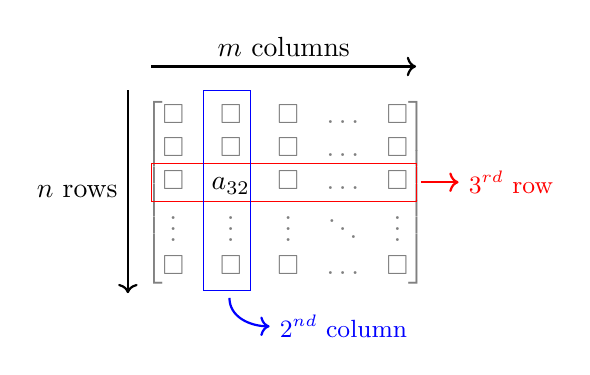
\begin{tikzpicture}[scale=0.6]
        \draw[thick, ->] (0,0) -- (0, -4.3) node[midway,left] {$n$ rows};
        \draw[thick, ->] (0.5,0.5) -- (6.1, 0.5) node[midway,above]{$m$ columns};
        %\node[xshift=-0.6cm,yshift=-1.3cm] {Rows};
        \node[gray,xshift=2.0cm,yshift=-1.3cm] {$\begin{bmatrix}
          \Box & \Box & \Box & \ldots & \Box \\
          \Box & \Box & \Box & \ldots & \Box \\
          \Box & \textcolor{black}{a_{32}} & \Box & \ldots & \Box \\
          \vdots & \vdots & \vdots & \ddots & \vdots \\
          \Box & \Box & \Box & \ldots & \Box \\
        \end{bmatrix}$};
        \draw[draw=red] (0.5,-2.35) rectangle ++(5.6,0.8);
        \draw[draw=blue] (1.6,-4.25) rectangle ++(1.0,4.25);
        \draw [thick, blue, ->] (2.15,-4.4) to [out=-90,in=180] (3.0, -5.0) node[right] {\small{$2^{nd}$ column}};
        \draw [thick, red, ->] (6.2,-1.95) to (7.,-1.95) node[right] {\small{$3^{rd}$ row}};
      \end{tikzpicture}\hspace{0.5cm}
    \end{center}
    \item Consider a matrix $A$ with $n$ rows and $m$ columns.$ \begin{cases} \text{\textbf{Tall/Skinny}} & n > m\\
      \text{\textbf{Square}} & n = m\\
      \text{\textbf{Wide/Fat}} & n < m\\
    \end{cases}$
  \end{itemize}
\end{frame}

\begin{frame}[t]{Matrices}
  \begin{itemize}
    \item $n$-vectors can be interpreted as $n \times 1$ matrices. These are called \textit{column vectors}.
    \item A matrix with only one row is called a \textit{row vector}, which can be referred to as $n$-row-vector.  $\mf{x} = \begin{bmatrix}1.45 & -3.1 & 12.4\end{bmatrix}$
    \item\textbf{Block matrices} \& \textbf{Submatrices}: $\mf{A} = \begin{bmatrix}
      \mf{B} & \mf{C} \\
      \mf{D} & \mf{E}
    \end{bmatrix}$.  What are the dimensions of the different matrices?
  \end{itemize}
\end{frame}


\begin{frame}[t]{Matrices}
  \begin{itemize}
    \item Matrices are also compact way to give a set of indexed column $n$-vectors, 
    $\mf{x}_1, \mf{x}_2, \mf{x}_3 \ldots \mf{x}_m$. 
    $$\mf{X} = \begin{bmatrix}
      \mf{x}_1 & \mf{x}_2 & \mf{x}_3 & \ldots & \mf{x}_m
    \end{bmatrix}$$
    
    \item \textbf{Zero matrix}$ = \mf{0}_{n\times m} = \begin{bmatrix}
      0 & 0 & \ldots & 0\\
      0 & 0 & \ldots & 0\\
      \vdots & \vdots & \ddots & \vdots\\
      0 & 0 & \ldots & 0
    \end{bmatrix}$
    
    \item \textbf{Identity matrix} is a square $n \times n$ matrix with all zero elements, except the diagonals where all elements are 1.
    $$i_{mn} = \begin{cases}
      1 & m = n\\
      0 & m \neq n
    \end{cases} \,\,\,\,\,\,\,\, \mf{I}_3=\begin{bmatrix}
      1 & 0 & 0\\
      0 & 1 & 0\\
      0 & 0 & 1\\
    \end{bmatrix} = \begin{bmatrix}
      \mf{e}_1 & \mf{e}_2 & \mf{e}_3
    \end{bmatrix}$$
  \end{itemize}
\end{frame}


\begin{frame}[t]{Matrices}
  \begin{itemize}
    
    \item \textbf{Diagonal matrices} is a square matrix with non-zero elements on its diagonal.
    $$\begin{bmatrix}
      0.4 & 0 & 0 & 0\\
      0 & -11 & 0 & 0\\
      0 & 0 & 21 & 0\\
      0 & 0 & 0 & 9.3\\
    \end{bmatrix} = \text{\textbf{diag}}\left(0.4, -11, 21, 9.3\right)$$
    \item \textbf{Triangular matrices}: Are square matrices. \textit{Upper triangular} $a_{ij} = 0, \forall i > j$; \textit{Lower triangular} $a_{ij} = 0, \forall i < j$.
  \end{itemize}
\end{frame}

\begin{frame}[t]{Matrix operations: Transpose}
  \begin{itemize}
    \item \textbf{Transpose} switches the rows and columns of a matrix. $\mf{A}$ is a $n\times m$ matrix, then its transpose is represented by $\mf{A}^{\top}$, which is a $m \times n$ matrix.
    \[ \mf{A} = \begin{bmatrix}
      a_{11} & a_{12} & a_{13}\\
      a_{21} & a_{22} & a_{23}\\
    \end{bmatrix} \implies \mf{A}^{\top} = \begin{bmatrix}
      a_{11} & a_{21}\\
      a_{12} & a_{22}\\
      a_{13} & a_{23}\\
    \end{bmatrix} \]
    Transpose converts between column and row vectors.\\
    What is the transpose of a block matrix? $\mf{A} = \begin{bmatrix}
      \mf{B} & \mf{C}\\\mf{D} & \mf{E}
    \end{bmatrix}$
  \end{itemize}
\end{frame}

\begin{frame}[t]{Matrix operations: Matrix Addition}
  \begin{itemize}
    \item \textbf{Matrix addition} can only be carried out with matrices of same size. Like vectors we perform element wise addition.
    \[ \begin{bmatrix}
      a_{11} & a_{12}\\
      a_{21} & a_{22}\\
    \end{bmatrix} + \begin{bmatrix}
      b_{11} & b_{12}\\
      b_{21} & b_{22}\\
    \end{bmatrix} = \begin{bmatrix}
      a_{11} + b_{11} & a_{12} + b_{12}\\
      a_{21} + b_{21} & a_{22} + b_{22}\\
    \end{bmatrix}\]
    
    \item \textbf{Properties of matrix addition}:
    \begin{itemize}
      \item \textit{Commutative}: $\mf{A} + \mf{B} = \mf{B} + \mf{A}$
      \item \textit{Associative}: $\left(\mf{A} + \mf{B}\right) + \mf{C} = \mf{A} + \left(\mf{B} + \mf{C}\right)$
      \item \textit{Addition with zero matrix}: $\mf{A} + \mf{0} = \mf{0} + \mf{A} = \mf{A}$
      \item \textit{Transpose of sum}: $\left(\mf{A} + \mf{B}\right)^{\top} = \mf{A}^{\top} + \mf{B}^{\top}$
    \end{itemize}
  \end{itemize}
\end{frame}

\begin{frame}[t]{Matrix operations: Scalar multiplication}
  \begin{itemize}
    \item \textbf{Scalar multiplication} Each element of the matrix gets multiplied by the scalar.
    \[ \alpha \begin{bmatrix}
      a_{11} & a_{12}\\
      a_{21} & a_{22}\\
    \end{bmatrix} = \begin{bmatrix}
      \alpha a_{11} & \alpha a_{12} \\
      \alpha a_{21} & \alpha a_{22} \\
    \end{bmatrix}\]
    \item We will mostly only deal with matrices with real entries. Such matrices are elements of the set $\mathbb{R}^{n\times m}$.
    \item Given the aforementioned matrix operations and their properties, is $\mathbb{R}^{n\times m}$ a vector space?
  \end{itemize}
\end{frame}

\begin{frame}[t]{Matrix operations: Matrix multiplication}
  \begin{itemize}
    \item A useful multiplication operation can be defined for matrices.
    \item It is possible to \textit{multiply} two matrices $\mf{A} \in \mathbb{R}^{n\times p}$ and $\mf{B} \in \mathbb{R}^{p\times m}$ through this \textit{matrix multiplication} procedure.
    \item The product matrix $\mf{C} \coloneqq \mf{A}\mf{B} \in \mathbb{R}^{n \times m}$, if the number of columns of $\mf{A}$ is equal to the number of rows of $\mf{B}$.
    \[ c_{ij} \coloneqq \sum_{k=1}^{p} a_{ik}b_{kj} \,\,\,\,\, \forall i \in \left\{1, \ldots n\right\}\,\,\, , j \in \left\{1 \ldots m\right\} \]
  \end{itemize}
\end{frame}

\begin{frame}[t]{Matrix multiplication}
  \begin{itemize}
    \item \textit{Inner product} is a special case of matrix multiplication between a \textit{row vector} and a \textit{column vector}.
    \[ \mf{x}^{\top}\mf{y} = \begin{bmatrix}
      x_1 \\ x_2 \\ \vdots \\x_n
    \end{bmatrix}^{\top}\begin{bmatrix}
      y_1 \\ y_2 \\ \vdots \\y_n
    \end{bmatrix} = \begin{bmatrix}
      x_1 & x_2 & \ldots &x_n
    \end{bmatrix}\begin{bmatrix}
      y_1 \\ y_2 \\ \vdots \\y_n
    \end{bmatrix} = \sum_{i=1}^nx_iy_i\]
  \end{itemize}
\end{frame}

\begin{frame}[t]{Matrix multiplication: Post-multiplication by a column vector}
  \begin{itemize}
    \item Consider a matrix $\mf{A} \in \mathbb{R}^{n \times m}$ and a $m$-vector $\mf{x} \in \mathbb{R}^m$. We can multiply $\mf{A}$ and $\mf{x}$ to obtain $\mf{y} = \mf{A}\mf{x} \in \mathbb{R}^n$.
    \[ \mf{y} = \begin{bmatrix}
      a_{11} & a_{12} & \ldots & a_{1m} \\
      a_{21} & a_{22} & \ldots & a_{2m} \\
      \vdots & \vdots & \ddots & \vdots \\
      a_{n1} & a_{n2} & \ldots & a_{nm} \\
    \end{bmatrix}\begin{bmatrix}
      x_1\\ x_2 \\ \vdots \\ x_{m}
    \end{bmatrix} = \begin{bmatrix}
      \sum_{i=1}^ma_{1i}x_i\\ \sum_{i=1}^ma_{2i}x_i \\ \vdots \\ \sum_{i=1}^ma_{ni}x_i
    \end{bmatrix} = \sum_{i=1}^mx_i\begin{bmatrix}
      a_{1i} \\ a_{2i} \\ \vdots \\ a_{ni}
    \end{bmatrix} = \sum_{i=1}^mx_i \mathbf{a}_{i} \]
    \item Post-multiplying a matrix $\mf{A}$ by a column vector $\mf{x}$ results in a linear combination of the columns of matrix $\mf{A}$.
    
    \item $\mathbf{x}$ provides the column mixture.
  \end{itemize}
\end{frame}

\begin{frame}[t]{Matrix multiplication: Pre-multiplication by a row vector}
  \begin{itemize}
    \item Let $\mf{x}^{\top} \in \mathbb{R}^{n}$ and $\mf{A} \in \mathbb{R}^{n \times m}$, then $\mf{y} = \mf{x}^{\top}\mf{A}$.
    \[ \mf{y} = \begin{bmatrix}
      x_1 & \ldots & x_n
    \end{bmatrix} \begin{bmatrix}
      a_{11} & \ldots & a_{1m} \\
      \vdots & \ddots & \vdots \\
      a_{n1} & \ldots & a_{nm} \\
    \end{bmatrix} = \begin{bmatrix} \sum_{i=1}^{n} x_i a_{i1} & \ldots & \sum_{i=1}^{n} x_i a_{im}
    \end{bmatrix} = \sum_{i=1}^n x_i \tilde{\mf{a}}_i^\top \]
    where, $\tilde{\mf{a}}_i^\top = \begin{bmatrix}
      a_{i1} & \ldots & a_{im}\end{bmatrix}$
      \item Pre-multiplying a matrix $\mf{A}$ by a row vector $\mf{x}$ results in a linear combination of the rows of $\mf{A}$.
      
      \item $\mf{x}^\top$ provides the row mixture.
  \end{itemize}
\end{frame}
  
\begin{frame}[t]{Matrix multiplication}
  \begin{itemize}
    \item Multiplying two matrices $\mf{A} \in \mathbb{R}^{n \times p}$ and $\mf{B} \in \mathbb{R}^{p \times m}$ produces $\mf{C} \in \mathbb{R}^{n \times m}$,
    \[ \mf{C} = \mf{A}\mf{B} = \begin{bmatrix}
      a_{11} & a_{12} & \ldots & a_{1p} \\
      a_{21} & a_{22} & \ldots & a_{2p} \\
      \vdots & \vdots & \ddots & \vdots \\
      a_{n1} & a_{n2} & \ldots & a_{np} \\
    \end{bmatrix} \begin{bmatrix}
      b_{11} & b_{12} & \ldots & b_{1m} \\
      b_{21} & b_{22} & \ldots & b_{2m} \\
      \vdots & \vdots & \ddots & \vdots \\
      b_{p1} & b_{p2} & \ldots & b_{pm} \\
    \end{bmatrix} = \begin{bmatrix}
      c_{11} & c_{12} & \ldots & c_{1m} \\
      c_{21} & c_{22} & \ldots & c_{2m} \\
      \vdots & \vdots & \ddots & \vdots \\
      c_{p1} & c_{n2} & \ldots & c_{nm} \\
    \end{bmatrix}\]
    
    \item \textbf{Four interpretations of matrix multiplication.}
    \begin{enumerate}
      \item Inner-Product interpretation
      \item Column interpretation
      \item Row interpretation
      \item Outer product interpretation.
    \end{enumerate} 
  \end{itemize}
\end{frame}

\begin{frame}[t]{Matrix multiplication: Inner-product Interpreation}
  \[ \mf{C} = \mf{A}\mf{B}, \,\,\, \mf{A} \in \mathbb{R}^{n \times p}, \, \mf{B} \in \mathbb{R}^{p \times m}, \, \mf{C} \in \mathbb{R}^{n \times m} \]
  \begin{itemize}
    \item $ij^{th}$ element of $\mf{C}$ is the inner product of the $i^{th}$ row of $\mf{A}$ and the $j^{th}$ column of $\mf{B}$.
    \[ c_{ij} = \sum_{k=1}^{m} a_{ik} b_{kj} = \tilde{\mf{a}}_i^{\top}\mf{b}_j \]
    where, $i \in \left\{1 \ldots n\right\}, j \in \left\{1 \ldots m\right\}$
  \end{itemize}
\end{frame}


\begin{frame}[t]{Matrix multiplication: Column interpretation}
  \[ \mf{C} = \mf{A}\mf{B}, \,\,\, \mf{A} \in \mathbb{R}^{n \times p}, \, \mf{B} \in \mathbb{R}^{p \times m}, \, \mf{C} \in \mathbb{R}^{n \times m} \]
  \begin{itemize}
    \item Columns of $\mf{C}$ are the linear combinations of the columns of $\mf{A}$.
    \[ \mf{C} = \mf{A} \begin{bmatrix}
      \mf{b}_{1} & \mf{b}_{2} & \ldots & \mf{b}_{m}
    \end{bmatrix} = \begin{bmatrix}
      \mf{A}\mf{b}_{1} & \mf{A}\mf{b}_{2} & \ldots & \mf{A}\mf{b}_{m}
    \end{bmatrix} \]
    
    \item $j^{th}$ column of $\mf{C}$ is the linear combination of the columns of $\mf{A}$
    \[ \mf{c}_j = \sum_{k=1}^{p} b_{kj} \mf{a}_k \]
  \end{itemize}
\end{frame}


\begin{frame}[t]{Matrix multiplication: Row interpretation}
  \[ \mf{C} = \mf{A}\mf{B}, \,\,\, \mf{A} \in \mathbb{R}^{n \times p}, \, \mf{B} \in \mathbb{R}^{p \times m}, \, \mf{C} \in \mathbb{R}^{n \times m} \]
  \begin{itemize}
    \item Rows of $\mf{C}$ are the linear combinations of the rows of $\mf{B}$.
    \[ \mf{C} = \begin{bmatrix}
      \tilde{\mf{a}}_{1}^\top \\ \tilde{\mf{a}}_{2}^\top \\ \ldots \\ \tilde{\mf{a}}_{n}^\top
    \end{bmatrix} \mf{B}  = \begin{bmatrix}
      \tilde{\mf{a}}_{1}^\top \mf{B} \\ \tilde{\mf{a}}_{2}^\top \mf{B} \\ \ldots \\ \tilde{\mf{a}}_{n}^\top \mf{B}
    \end{bmatrix} \]
    
    \item $i^{th}$ row of $\mf{C}$ is the linear combination of the rows of $\mf{B}$
    \[ \tilde{\mf{c}}_i^\top = \sum_{k=1}^{p} a_{ik} \tilde{\mf{b}}_{k}^\top  \]
  \end{itemize}
\end{frame}


\begin{frame}[t]{Matrix multiplication: Outer product interpretation}
  \begin{itemize}
    \item \textbf{Outer product}: Product between a colum vector and a row vector. Let $\mf{x} \in \mathbb{R}^n$ and $\mf{y} \in \mathbb{R}^m$. The \textit{outer product} is defined as,
    \[ \mf{x}\mf{y}^{\top} = \begin{bmatrix}
      x_1\\ x_2\\ \vdots \\x_n
    \end{bmatrix} \begin{bmatrix}
      y_1 &  y_2 & \cdots & y_m
    \end{bmatrix} = \begin{bmatrix}
      x_1y_1 &  x_1y_2 & \cdots & x_1y_m \\
      x_2y_1 &  x_2y_2 & \cdots & x_2y_m \\
      \vdots &  \vdots & \ddots & \vdots \\
      x_ny_1 &  x_ny_2 & \cdots & x_ny_m \\
    \end{bmatrix} \in \mb{R}^{n \times m} \]
  \end{itemize}
\end{frame}


\begin{frame}[t]{Matrix multiplication: Outer product interpretation}
  \[ \mf{C} = \mf{A}\mf{B}, \,\,\, \mf{A} \in \mathbb{R}^{n \times p}, \, \mf{B} \in \mathbb{R}^{p \times m}, \, \mf{C} \in \mathbb{R}^{n \times m} \]
  \begin{itemize}
    \item $\mf{C}$ can be written as the sum of $p$ outer products of columns of $\mf{A}$ and rows of $\mf{B}$.
    \[ \mf{C} = \mf{A}\mf{B} = \begin{bmatrix}
      \mf{a}_1 & \mf{a}_2 & \mf{a}_3 & \ldots & \mf{a}_p
    \end{bmatrix} \begin{bmatrix}
      \tilde{\mf{b}}_1^{\top} \\
      \tilde{\mf{b}}_2^{\top} \\
      \tilde{\mf{b}}_3^{\top} \\
      \vdots \\
      \tilde{\mf{b}}_p^{\top}
    \end{bmatrix} = \sum_{i=1}^{p}\mf{a}_i\tilde{\mf{b}}_i^{\top} \]
  \end{itemize}
\end{frame}


\begin{frame}[t]{Properties of matrix multiplication}
  \begin{itemize}
    \item \textbf{Not commutative}: $\mf{A}\mf{B} \neq \mf{B}\mf{A}$\\
    The product of two matrices might not alwasys be defined. When it is defined, $\mf{A}\mf{B}$ and $\mf{B}\mf{A}$ need not match.
    \item \textbf{Distributive}:  $\mf{A}\left(\mf{B} + \mf{C}\right) = \mf{A}\mf{B} + \mf{B}\mf{C}$ and $\left(\mf{A} + \mf{B}\right)\mf{C} = \mf{A}\mf{C} + \mf{B}\mf{C}$ 
    \item \textbf{Associative}: $\mf{A}\left(\mf{B}\mf{C}\right) = \left(\mf{A}\mf{B}\right)\mf{C} $
    \item \textbf{Transpose}: $\left(\mf{A}\mf{B}\right)^{\top} = \mf{B}^{\top}\mf{A}^{\top}$
    \item \textbf{Scalar product}: $\alpha\left(\mf{A}\mf{B}\right) = \left(\alpha \mf{A}\right)\mf{B} = \mf{A}\left(\alpha \mf{B}\right)$
  \end{itemize}
\end{frame}


\begin{frame}[t]{Linear transformations}
  \begin{itemize}
    \item Linear functions $f: \mathbb{R}^m \mapsto \mathbb{R}$, 
    \[ y = f\left(\mf{x}\right) = \mf{w}^{\top}\mf{x}; \,\,\, \mf{w}, \mf{x} \in \mathbb{R}^m, \,\, y \in \mathbb{R} \]
    
    \item Generalization of the linear function is when its range $\mathbb{R}^n$:
    \[ \mf{y} = f\left(\mf{x}\right); \,\,\, \mf{x} \in \mathbb{R}^m, \,\, \mf{y} \in \mathbb{R}^n \]
    
    \item These can be represented as, $\mf{y} = \mf{Ax}, \,\,\, \mf{A} \in \mathbb{R}^{n \times m}$.\\
    
    \item Matrices can be thought of as representing a particular linear transformation.
  \end{itemize}
\end{frame}


\begin{frame}[t]{Why does matrix multiplication have this strange definition?}
  Consider the following two functions,
  \begin{small}
    \[ \mf{y} = f\lp\mf{x}\rp = \mf{A}\mf{x} \longrightarrow \begin{bmatrix}y_1 \\ y_2\end{bmatrix} = f\left(\begin{bmatrix}x_1 \\ x_2\end{bmatrix}\right) = \begin{bmatrix}ax_1 + bx_2 \\ cx_1 + dx_2\end{bmatrix} = \begin{bmatrix}a & b \\ c & d\end{bmatrix}\begin{bmatrix}x_1 \\ x_2\end{bmatrix}\]
    \[ \mf{v} = g\lp\mf{u}\rp = \mf{B}\mf{u} \longrightarrow \begin{bmatrix}v_1 \\ v_2\end{bmatrix} = g\left(\begin{bmatrix}u_1 \\ u_2\end{bmatrix}\right) = \begin{bmatrix}\alpha u_1 + \beta u_2 \\ \gamma u_1 + \delta u_2\end{bmatrix} = \begin{bmatrix}\alpha & \beta \\ \gamma & \delta\end{bmatrix}\begin{bmatrix}u_1 \\ u_2\end{bmatrix}\]
    \[ \begin{split}
      \mf{z} = h\left(\mf{u}\right) &= f\left(g\left(\mf{u}\right)\right) = f\left(\begin{bmatrix}\alpha u_1 + \beta u_2 \\ \gamma u_1 + \delta u_2\end{bmatrix}\right) = \begin{bmatrix}a\alpha u_1 + a\beta u_2 + b\gamma u_1 + b\delta u_2 \\ c\alpha u_1 + c\beta u_2 + d\gamma u_1 + d\delta u_2 \end{bmatrix}\\
      &= \begin{bmatrix}\left(a\alpha + b\gamma\right) u_1 + \left(a\beta + b\delta\right)u_2 \\ \left(c\alpha + d\gamma\right)u_1  + \left(c\beta + d\delta\right)u_2 \end{bmatrix} = \begin{bmatrix}a\alpha + b\gamma & a\beta + b\delta \\ c\alpha + d\gamma & c\beta + d\delta \end{bmatrix} \begin{bmatrix}u_1 \\ u_2 \end{bmatrix}
    \end{split}
    \]
    \[\mf{z} = \mf{A}\lp\mf{B}\mf{u}\rp = \lp\mf{A}\mf{B}\rp\mf{u} \implies \mf{A}\mf{B} = \begin{bmatrix}a & b \\ c & d\end{bmatrix}\begin{bmatrix}\alpha & \beta \\ \gamma & \delta\end{bmatrix} = \begin{bmatrix}a\alpha + b\gamma & a\beta + b\delta \\ c\alpha + d\gamma & c\beta + d\delta \end{bmatrix}
    \]
  \end{small}
  Matrix multiplication represents the composition of linear transformations.
\end{frame}


\begin{frame}[t]{Rank of a matrix $\mf{A}$}
  \begin{itemize}
    \item \textbf{Rank of a matrix $\mf{A}$}: dimension of the subspace spanned by the columns of $\mf{A}$ or the rows of $\mf{A} \in \mb{R}^{n \times m}$. 
    \[ \begin{split} 
      rank\lp \mf{A} \rp &= \mathrm{dim} \, span\lp \lc \mf{a}_1, \mf{a}_2, \ldots \mf{a}_m \rc \rp \rightarrow \text{Column rank}\\ 
      &= \mathrm{dim} \, span\lp \lc \tilde{\mf{a}}_1^\top, \tilde{\mf{a}}_2^\top, \ldots \tilde{\mf{a}}_n^\top \rc \rp \rightarrow \text{Row rank}
    \end{split}
    \]
    
    \item Column Rank is always equal to the row rank.
    
    \item Rank tells us the number of independent columns/row in the matrix.
    
    \item \textbf{Full rank matrix } $\mf{A}$: $rank\lp \mf{A} \rp  = \min\lp n, m\rp$\\
    \textbf{Rank deficient matrix } $\mf{A}$: $rank\lp \mf{A} \rp  < \min\lp n, m\rp$
  \end{itemize}
\end{frame}

\begin{frame}[t]{Matrix Inverse}
  \begin{small}
    \begin{itemize}
      \item Consider the square matrix $\mf{A} \in \mathbb{R}^{n \times n}$. $\mf{B} \in \mathbb{R}^{n \times n}$ is the inverse of $\mf{A}$, if $\mf{AB} = \mf{BA} = \mf{I}_n$, and $\mf{B}$ is represented as $\mf{A}^{-1}$.
      \item Not all matrices have inverses. A matrix with an inverse is called \textbf{non-singular}, otherwise it is called \textbf{singular}.
      \item For a non-singular matrix $\mf{A}$, $\mf{A}^{-1}$ is unique. $\mf{A}^{-1}$ is both the left and right inverse.
      \item A matrix $\mf{A}$ has an inverse, if and only if $\mf{A}$ is full rank, i.e. $rank\left(\mf{A}\right) = n$
      \item $\mf{Ax} = \mf{b}$ can be solved as follows, $\mf{x} = \mf{A}^{-1}\mf{b}$. \textit{It is never solved like this in practice.}
      \item Inverse of product of matrices, $\left(\mf{AB}\right)^{-1} = \mf{B}^{-1}\mf{A}^{-1}$.
      \item $\left(\mf{A}^{-1}\right)^{-1} = \mf{A}$ and $\left(\mf{A}^{-1}\right)^{\top} = \left(\mathbf{A}^{\top}\right)^{-1}$
    \end{itemize}
  \end{small}
\end{frame}


\begin{frame}[t]{Representation of vectors in a basis}
  \begin{itemize}
  \item Consider the vector space $\mb{R}^n$ with basis $\left\{\mf{v}_1, \mf{v}_2, \ldots \mf{v}_n\right\}$. Any vector in $\mf{b} \in \mb{R}^n$ can be representated as a linear combination of $\mf{v}_i$s,
  \[ \mf{b} = \sum_{i=1}^{n} \mf{v}_i\mf{a}_i = \mf{V}\mf{a}; \,\,\, \mf{a} \in \mb{R}^n, \,\,\, \mf{V} = \begin{bmatrix*}\mf{v}_1 & \mf{v}_2 & \cdots & \mf{v}_n\end{bmatrix*} \in \mb{R}^{n \times n} \]
  
    \begin{center}
    \begin{minipage}{.3\textwidth}
    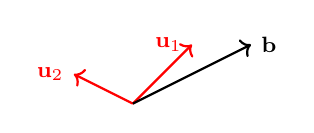
\begin{tikzpicture}[scale=0.75]
      \draw[red,thick,->] (0, 0) -- (1, 1) node[red, above, left]{{\footnotesize $\mf{u}_1$}};
      \draw[red,thick,->] (0, 0) -- (-1, 0.5) node[red, above, left]{{\footnotesize $\mf{u}_2$}};
      \draw[black,thick,->] (0, 0) -- (2, 1) node[black, above, right]{{\footnotesize $\mf{b}$}};
    \end{tikzpicture}
    \end{minipage}
    \begin{minipage}{.3\textwidth}
    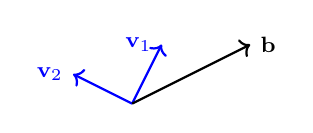
\begin{tikzpicture}[scale=0.75]
      \draw[blue,thick,->] (0, 0) -- (0.5, 1) node[blue, above, left]{{\footnotesize $\mf{v}_1$}};
      \draw[blue,thick,->] (0, 0) -- (-1, 0.5) node[blue, above, left]{{\footnotesize $\mf{v}_2$}};
      \draw[black,thick,->] (0, 0) -- (2, 1) node[black, above, right]{{\footnotesize $\mf{b}$}};
    \end{tikzpicture}
    \end{minipage}
    \begin{minipage}{.3\textwidth}
    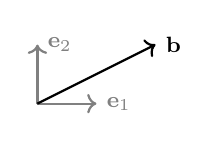
\begin{tikzpicture}[scale=0.75]
      \draw[gray,thick,->] (0, 0) -- (1, 0) node[gray, above, right]{{\footnotesize $\mf{e}_1$}};
      \draw[gray,thick,->] (0, 0) -- (0, 1) node[gray, above, right]{{\footnotesize $\mf{e}_2$}};
      \draw[black,thick,->] (0, 0) -- (2, 1) node[black, above, right]{{\footnotesize $\mf{b}$}};
    \end{tikzpicture}
    \end{minipage}
    \end{center}
    $\left\{\mf{v}_1, \mf{v}_2\right\}$, $\left\{\mf{u}_1, \mf{u}_2\right\}$ and $\left\{\mf{e}_1, \mf{e}_2\right\}$ are valid basis for $\mb{R}^2$, and the presentation for $\mf{b}$ in each one of them is different.
  \end{itemize}
\end{frame}


\begin{frame}[t]{Matrix Inverse}
\begin{itemize}
    \item Consider the equation $\mf{Ax} = \mf{y}$, where $\mf{A} \in \mb{R}^{n \times n}$ and $\mf{x}, \mf{y} \in \mb{R}^n$. 

    \item Assume $\mf{A}$ is non-singular $\implies$ columns of $\mf{A}$, $\lc \mf{a}_1, \mf{a}_2, \cdots \mf{a}_n\rc$, represent a basis for $\mb{R}^n$.

    \item Then $\mf{x}$ represents $\mf{y}$ in the basis consisitng of the columns of $\mf{A}$.
    \[ \mf{y} = \mf{Ax} = \sum_{i=1}^{n}\mf{a}_i x_i \implies \,\, \mf{x} = \mf{A}^{-1}\mf{y} = \begin{bmatrix*}\tilde{\mf{b}}_1^\top \\ \tilde{\mf{b}}_2^\top \\ \vdots \\ \tilde{\mf{b}}_n^\top\end{bmatrix*}\mf{y} = \begin{bmatrix*}\tilde{\mf{b}}_1^\top\mf{y} \\ \tilde{\mf{b}}_2^\top\mf{y} \\ \vdots \\ \tilde{\mf{b}}_n^\top\mf{y}\end{bmatrix*} \]
    \item $\mf{A}^{-1}$ is the matrix that allows change of basis to the columns of $\mf{A}$ from the standard basis!
  \end{itemize}
\end{frame}


\begin{frame}{Some more definitions and conventions}
  When studying kinematics we will always assume the following:
  \begin{itemize}
    \item \textbf{Fixed frame} $F$: This is a stationary frame of reference attached to the corner of a room, the base of a robot, etc.
    \item \textbf{Body frame} $B$: A frame attached to a rigid body of interest. E.g. frame of a robot's moving link, frame on a mobile robot's chasis, etc.
    \item All frames are assumed to be right-handed frames. If $\mf{x}$ and $\mf{y}$ are the x and x axes of a referene frame, then $\mf{z} = \mf{x} \times \mf{y}$, where `$\times$' is the cross product between two vectors.
  \end{itemize}
\end{frame}


\begin{frame}{Rigid Body Motions in a Plane: Rotation}
  \begin{columns}[T]
    \begin{column}{0.475\textwidth}
      Let \rbframe{s} and \rbframe{b} be the fixed and body frames respectively. The body frame is rotated by an angle $\theta$ with respect to the fixed frame.

      The vectors $\lc \mf{x}_{s}, \mf{y}_s \rc$ and $\lc \mf{x}_b, \mf{y}_b \rc$ form an orthonormal basis for \rbframe{s} and \rbframe{b}, respectively.

      $\bullet$ Representation of $\mf{x}_b$ in \rbframe{s}: $\bmx \mf{x}_s^\top \mf{x}_b \\ \mf{y}_s^\top \mf{x}_b \emx$
      \vspace{0.2cm}

      $\bullet$ Representation of $\mf{y}_b$ in \rbframe{s}: $\bmx \mf{x}_s^\top \mf{y}_b \\ \mf{y}_s^\top \mf{y}_b \emx$

    \end{column}
    \begin{column}{0.5\textwidth}
      \begin{figure}
        \centering
        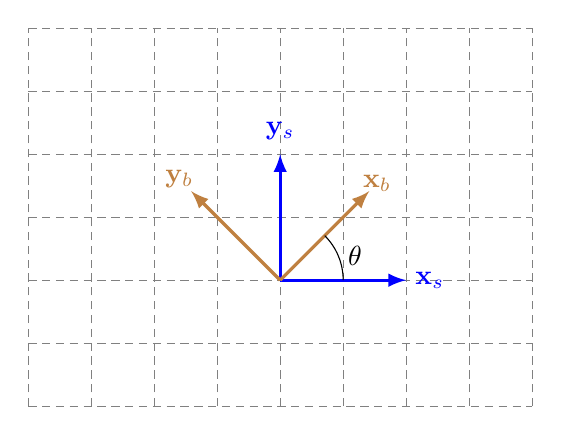
\begin{tikzpicture}[scale=8]
          \foreach \x in {-0.4, -0.3, -0.2, -0.1, 0, 0.1, 0.2, 0.3, 0.4}
            \draw[gray, thin, densely dashed] (\x,-0.2)--(\x,0.4);
          \foreach \x in {-0.2, -0.1, 0, 0.1, 0.2, 0.3, 0.4}
            \draw[gray, thin, densely dashed] (-0.4,\x)--(0.4,\x);
          \draw[very thick, blue, -latex] (0,0) -- (0.2,0) node[xshift=0.3cm, yshift=0cm]{$\mf{x}_s$};
          \draw[very thick, blue, -latex] (0,0) -- (0,0.2) node[xshift=0cm, yshift=0.3cm]{$\mf{y}_s$};
          \draw[very thick, brown, -latex] (0, 0) -- (0.1414,0.1414) node[xshift=0.1cm, yshift=0.1cm]{$\mf{x}_b$};
          \draw[very thick, brown, -latex] (0, 0) -- (-0.1414, 0.1414) node[xshift=-0.15cm, yshift=0.15cm]{$\mf{y}_b$};
          % Draw a radius
          \draw (0,0) ++ (0.1,0) arc (0:45:0.1) node[midway, right]{$\theta$};
        \end{tikzpicture}
      \end{figure}
    \end{column}
  \end{columns}
\end{frame}


\begin{frame}{Rigid Body Motions in a Plane: Rotation}
  \begin{columns}[T]
    \begin{column}{0.475\textwidth}
      This representation can be compactly expressed as the following,
      \[ \bmx \mf{x}_s^\top \mf{x}_b & \mf{x}_s^\top \mf{y}_b \\ \mf{y}_s^\top \mf{x}_b & \mf{y}_s^\top \mf{y}_b \emx \triangleq \mf{R}_{sb}\]

      From the definition of the standard inner product, we know that,
      \[  \mf{R}_{sb} = \bmx \cos\theta & \sin\theta \\ -\sin\theta & \cos\theta \emx \]

      $\mf{R}_{sb}$ is rotation matrix representing \rbframe{b} in \rbframe{s}. It is parametrized by a single parameter $\theta$.

    \end{column}
    \begin{column}{0.5\textwidth}
      \begin{figure}
        \centering
        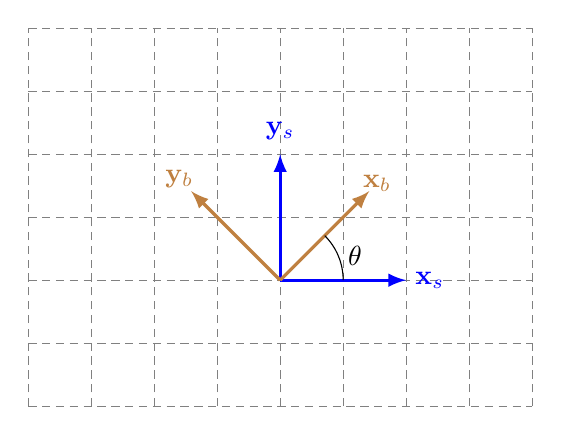
\begin{tikzpicture}[scale=8]
          \foreach \x in {-0.4, -0.3, -0.2, -0.1, 0, 0.1, 0.2, 0.3, 0.4}
            \draw[gray, thin, densely dashed] (\x,-0.2)--(\x,0.4);
          \foreach \x in {-0.2, -0.1, 0, 0.1, 0.2, 0.3, 0.4}
            \draw[gray, thin, densely dashed] (-0.4,\x)--(0.4,\x);
          \draw[very thick, blue, -latex] (0,0) -- (0.2,0) node[xshift=0.3cm, yshift=0cm]{$\mf{x}_s$};
          \draw[very thick, blue, -latex] (0,0) -- (0,0.2) node[xshift=0cm, yshift=0.3cm]{$\mf{y}_s$};
          \draw[very thick, brown, -latex] (0, 0) -- (0.1414,0.1414) node[xshift=0.1cm, yshift=0.1cm]{$\mf{x}_b$};
          \draw[very thick, brown, -latex] (0, 0) -- (-0.1414, 0.1414) node[xshift=-0.15cm, yshift=0.15cm]{$\mf{y}_b$};
          % Draw a radius
          \draw (0,0) ++ (0.1,0) arc (0:45:0.1) node[midway, right]{$\theta$};
        \end{tikzpicture}
      \end{figure}
    \end{column}
  \end{columns}
\end{frame}


\begin{frame}{Rigid Body Motions in a Plane: Rotation}
  \begin{columns}[T]
    \begin{column}{0.575\textwidth}
      All 2D Rotaiton matrices $\mf{R} \in \mb{R}^{2 \times 2}$ are orthogonal matrices, i.e. $\mf{R}^{-1} = \mf{R}^\top$.

      Rotation matrices have three different purposes:
      \vspace{1cm}

      \tikz[baseline=(char.base)]{\node[shape=circle,draw,inner sep=2pt] (char) {\textbf{1}};} \textcolor{myred}{$\mf{R}_{sb}$: Represents the orientation of \rbframe{b} in \rbframe{s}.}

    \end{column}
    \begin{column}{0.4\textwidth}
      \begin{figure}
        \centering
        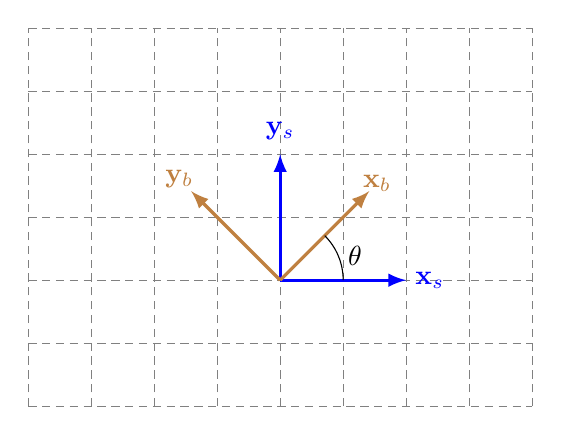
\begin{tikzpicture}[scale=8]
          \foreach \x in {-0.4, -0.3, -0.2, -0.1, 0, 0.1, 0.2, 0.3, 0.4}
            \draw[gray, thin, densely dashed] (\x,-0.2)--(\x,0.4);
          \foreach \x in {-0.2, -0.1, 0, 0.1, 0.2, 0.3, 0.4}
            \draw[gray, thin, densely dashed] (-0.4,\x)--(0.4,\x);
          \draw[very thick, blue, -latex] (0,0) -- (0.2,0) node[xshift=0.3cm, yshift=0cm]{$\mf{x}_s$};
          \draw[very thick, blue, -latex] (0,0) -- (0,0.2) node[xshift=0cm, yshift=0.3cm]{$\mf{y}_s$};
          \draw[very thick, brown, -latex] (0, 0) -- (0.1414,0.1414) node[xshift=0.1cm, yshift=0.1cm]{$\mf{x}_b$};
          \draw[very thick, brown, -latex] (0, 0) -- (-0.1414, 0.1414) node[xshift=-0.15cm, yshift=0.15cm]{$\mf{y}_b$};
          % Draw a radius
          \draw (0,0) ++ (0.1,0) arc (0:45:0.1) node[midway, right]{$\theta$};
        \end{tikzpicture}
      \end{figure}
    \end{column}
  \end{columns}
\end{frame}


\begin{frame}{Rigid Body Motions in a Plane: Rotation}
  \begin{columns}[T]
    \begin{column}{0.575\textwidth}
      Rotation matrices have three different purposes:
      \vspace{0.25cm}

      \tikz[baseline=(char.base)]{\node[shape=circle,draw,inner sep=2pt] (char) {\textbf{2}};} \textcolor{myred}{
        Transforming vectors between reference frames.
        \[ \mf{v}_s = \mf{R}_{sb}\mf{v}_b \quad \mf{v}_b = \mf{R}_{bs}\mf{v}_s  = \mf{R}_{sb}^\top\mf{v}_s \]
      }
      
      \textcolor{mygray}{\small Note that the second letter in the subscript of the rotation matrix on left gets cancelled by the first letter in the subscript of the vector on the right.
      \[ \mf{v}_l = \mf{R}_{l\cancel{m}} \mf{v}_{\cancel{m}} \]}

    \end{column}
    \begin{column}{0.4\textwidth}
      \begin{figure}
        \centering
        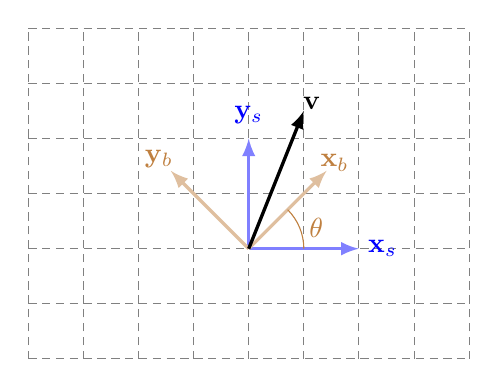
\begin{tikzpicture}[scale=7]
          \foreach \x in {-0.4, -0.3, -0.2, -0.1, 0, 0.1, 0.2, 0.3, 0.4}
            \draw[gray, thin, densely dashed] (\x,-0.2)--(\x,0.4);
          \foreach \x in {-0.2, -0.1, 0, 0.1, 0.2, 0.3, 0.4}
            \draw[gray, thin, densely dashed] (-0.4,\x)--(0.4,\x);
          \draw[very thick, blue!50!, -latex] (0,0) -- (0.2,0) node[xshift=0.3cm, yshift=0cm, text=blue]{$\mf{x}_s$};
          \draw[very thick, blue!50!, -latex] (0,0) -- (0,0.2) node[xshift=0cm, yshift=0.3cm, text=blue]{$\mf{y}_s$};
          \draw[very thick, brown!50!, -latex] (0, 0) -- (0.1414,0.1414) node[xshift=0.1cm, yshift=0.1cm, text=brown]{$\mf{x}_b$};
          \draw[very thick, brown!50!, -latex] (0, 0) -- (-0.1414, 0.1414) node[xshift=-0.15cm, yshift=0.15cm, text=brown]{$\mf{y}_b$};
          \draw[very thick, black, -latex] (0, 0) -- (0.1,0.25) node[xshift=0.1cm, yshift=0.1cm]{$\mf{v}$};
          % Draw a radius
          \draw[brown] (0,0) ++ (0.1,0) arc (0:45:0.1) node[midway, right]{$\theta$};
        \end{tikzpicture}
      \end{figure}
    \end{column}
  \end{columns}
\end{frame}


\begin{frame}{Rigid Body Motions in a Plane: Rotation}
  \begin{columns}[T]
    \begin{column}{0.575\textwidth}
      Rotation matrices have three different purposes:
      \vspace{1cm}

      \tikz[baseline=(char.base)]{\node[shape=circle,draw,inner sep=2pt] (char) {\textbf{3}};} \textcolor{myred}{
        Rotate a vector  $\mf{w}_s$ by an angle $\theta$ about the origin.
        \[ \mf{w}_s' = \mf{R}_{sb}\mf{w}_s \]
      }
    \end{column}
    \begin{column}{0.4\textwidth}
      \begin{figure}
        \centering
        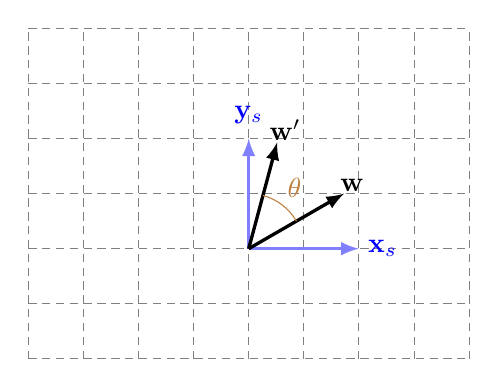
\begin{tikzpicture}[scale=7]
          \foreach \x in {-0.4, -0.3, -0.2, -0.1, 0, 0.1, 0.2, 0.3, 0.4}
            \draw[gray, thin, densely dashed] (\x,-0.2)--(\x,0.4);
          \foreach \x in {-0.2, -0.1, 0, 0.1, 0.2, 0.3, 0.4}
            \draw[gray, thin, densely dashed] (-0.4,\x)--(0.4,\x);
          \draw[very thick, blue!50!, -latex] (0,0) -- (0.2,0) node[xshift=0.3cm, yshift=0cm, text=blue]{$\mf{x}_s$};
          \draw[very thick, blue!50!, -latex] (0,0) -- (0,0.2) node[xshift=0cm, yshift=0.3cm, text=blue]{$\mf{y}_s$};
          \draw[very thick, black, -latex] (0,0) -- (30:0.2) node[xshift=0.1cm, yshift=0.1cm]{$\mf{w}$};
          \draw[very thick, black, -latex] (0,0) -- (75:0.2) node[xshift=0.1cm, yshift=0.15cm]{$\mf{w}'$};
          % Draw a radius
          \draw[brown] (0,0) ++ (30:0.1) arc (30:75:0.1) node[yshift=0.1cm, xshift=0.4cm]{$\theta$};
        \end{tikzpicture}
      \end{figure}
    \end{column}
  \end{columns}
\end{frame}


\begin{frame}{Rigid Body Motions in a Plane: Rotation}
  \begin{columns}[T]
    \begin{column}{0.575\textwidth}
      Consider two body reference frames \rbframe{b_1} and \rbframe{b_2}. Let $\mf{R}_{sb_1}$ \rbframe{b_1} in \rbframe{s}. And let $\mf{R}_{b_1b_2}$ be the rotation matrix representing \rbframe{b_2} in \rbframe{b_1}. Then,

      \[ \mf{R}_{sb_2} = \mf{R}_{s\cancel{b_1}}\mf{R}_{\cancel{b_1}b_2} \]

      Show that:
      \[ \mf{R}_{b_1b_2} = \bmx \cos\lp \theta_1 + \theta_2 \rp & \sin\lp \theta_1 + \theta_2 \rp \\ -\sin\lp \theta_1 + \theta_2 \rp & \cos\lp \theta_1 + \theta_2 \rp \emx \]

    \end{column}
    \begin{column}{0.4\textwidth}
      \begin{figure}
        \centering
        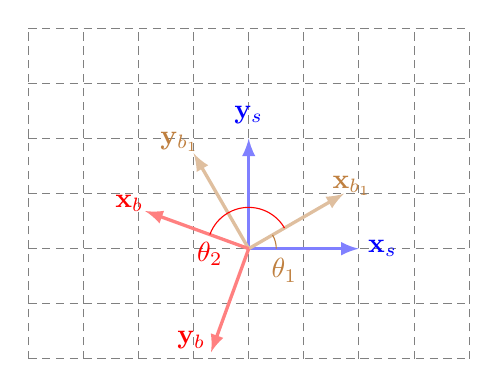
\begin{tikzpicture}[scale=7]
          \foreach \x in {-0.4, -0.3, -0.2, -0.1, 0, 0.1, 0.2, 0.3, 0.4}
            \draw[gray, thin, densely dashed] (\x,-0.2)--(\x,0.4);
          \foreach \x in {-0.2, -0.1, 0, 0.1, 0.2, 0.3, 0.4}
            \draw[gray, thin, densely dashed] (-0.4,\x)--(0.4,\x);
          % Space frame
          \draw[very thick, blue!50!, -latex] (0,0) -- (0.2,0) node[xshift=0.3cm, yshift=0cm, text=blue]{$\mf{x}_s$};
          \draw[very thick, blue!50!, -latex] (0,0) -- (0,0.2) node[xshift=0cm, yshift=0.3cm, text=blue]{$\mf{y}_s$};
          % Body frame 1
          \draw[very thick, brown!50!, -latex] (0, 0) -- ({0.2*cos(30)},{0.2*sin(30)}) node[xshift=0.1cm, yshift=0.1cm, text=brown]{$\mf{x}_{b_1}$};
          \draw[very thick, brown!50!, -latex] (0, 0) -- ({-0.2*sin(30)},{0.2*cos(30)}) node[xshift=-0.175cm, yshift=0.15cm, text=brown]{$\mf{y}_{b_1}$};
          % Body frame 2
          \draw[very thick, red!50!, -latex] (0, 0) -- ({0.2*cos(160)},{0.2*sin(160)}) node[xshift=-0.2cm, yshift=0.1cm, text=red]{$\mf{x}_b$};
          \draw[very thick, red!50!, -latex] (0, 0) -- ({-0.2*sin(160)},{0.2*cos(160)}) node[xshift=-0.25cm, yshift=0.15cm, text=red]{$\mf{y}_b$};
          % Draw a radius
          \draw[brown] (0,0) ++ (0.05,0) arc (0:30:0.05) node[xshift=0.15cm, yshift=-0.45cm]{$\theta_1$};
          \draw[red, thin] (30:0.075) arc (30:160:0.075) node[xshift=0.cm, yshift=-0.25cm]{$\theta_2$};
        \end{tikzpicture}
      \end{figure}
    \end{column}
  \end{columns}
\end{frame}


\begin{frame}{Rigid Body Motions in a Plane: Rotation and Translation}
  \begin{columns}[T]
    \begin{column}{0.475\textwidth}
      What do we do when have the body frame \rbframe{b} translated by a vector $\mf{p}_{sb}$ and rotated by a certain angle with repsect to the space frame \rbframe{s}?

      \textcolor{mygray}{\small \textbf{Note}: $\mf{p}_{sb}$ is the representation of the position of the origin of \rbframe{b} with respect to the \rbframe{s}.}

      Let $\mf{R}_{sb}$ be the represntation of \rbframe{b} in \rbframe{s}. Then, the complete representation of \rbframe{b} in \rbframe{s} is given by the pair $\lp \mf{R}_{sb}, \mf{p}_{sb}\rp$.
      \[ \mf{p}_{sb} = \bmx p_{{sb}_x} \\ p_{{sb}_y} \emx \quad \quad \mf{R}_{sb} = \bmx \cos\theta  & \sin\theta \\ -
      \sin\theta & \cos\theta \emx \]
      
    \end{column}
    \begin{column}{0.5\textwidth}
      \begin{figure}
        \centering
        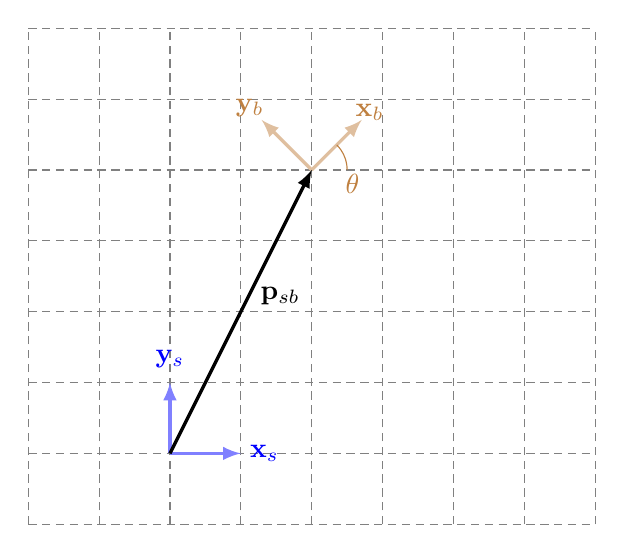
\begin{tikzpicture}[scale=4.5]
          \foreach \x in {-0.4, -0.2, 0, 0.2, 0.4, 0.6, 0.8, 1.0, 1.2}
            \draw[gray, thin, densely dashed] (\x,-0.2)--(\x,1.2);
          \foreach \x in {-0.2, 0, 0.2, 0.4, 0.6, 0.8, 1.0, 1.2}
            \draw[gray, thin, densely dashed] (-0.4,\x)--(1.2,\x);
          \draw[very thick, blue!50!, -latex] (0,0) -- (0.2,0) node[xshift=0.3cm, yshift=0cm, text=blue]{$\mf{x}_s$};
          \draw[very thick, blue!50!, -latex] (0,0) -- (0,0.2) node[xshift=0cm, yshift=0.3cm, text=blue]{$\mf{y}_s$};
          \draw[very thick, brown!50!, -latex] (0.4,0.8) -- (0.5414,0.9414) node[xshift=0.1cm, yshift=0.1cm, text=brown]{$\mf{x}_b$};
          \draw[very thick, brown!50!, -latex] (0.4,0.8) -- (0.2586, 0.9414) node[xshift=-0.15cm, yshift=0.15cm, text=brown]{$\mf{y}_b$};
          \draw[very thick, black, -latex] (0,0) -- (0.4,0.8) node[xshift=-0.4cm, yshift=-1.6cm]{$\mf{p}_{sb}$};
          \draw[brown] (0,0) ++ (0.5,0.8) arc (0:45:0.1) node[xshift=0.2cm, yshift=-0.5cm]{$\theta$};
        \end{tikzpicture}
      \end{figure}
    \end{column}
  \end{columns}
\end{frame}


\begin{frame}{Rigid Body Motions in a Plane: Rotation and Translation}
  \begin{columns}[T]
    \begin{column}{0.475\textwidth}
      Consider the point represented by the small black circle, whose position is given by $\mf{v}_{s}$ and $\mf{v}_{b}$ in \rbframe{s} and \rbframe{b}, respectively. The transformation between $\mf{v}_{s}$ and $\mf{v}_{b}$ is given by ,
      \[ \mf{v}_{s} = \mf{R}_{sb}\mf{v}_b + \mf{p}_{sb} \]
      \[ \begin{split}
          \mf{v}_{b} &= \mf{R}_{sb}^\top\lp \mf{v}_s - \mf{p}_{sb} \rp \\
                     &= \mf{R}_{bs} \mf{v}_s - \mf{R}_{bs} \mf{p}_{sb} \\
                     &= \mf{R}_{bs} \mf{v}_s + \mf{p}_{bs}
         \end{split} 
        \]
      $\lp \mf{R}_{sb}, \mf{p}_{sb}\rp$ transforms \rbframe{b} $\mapsto$ \rbframe{s}.
      
      $\lp \mf{R}_{sb}^\top, -\mf{R}_{sb}^\top\mf{p}_{sb}\rp$ transforms \rbframe{s} $\mapsto$ \rbframe{b}.
    \end{column}
    \begin{column}{0.5\textwidth}
      \begin{figure}
        \centering
        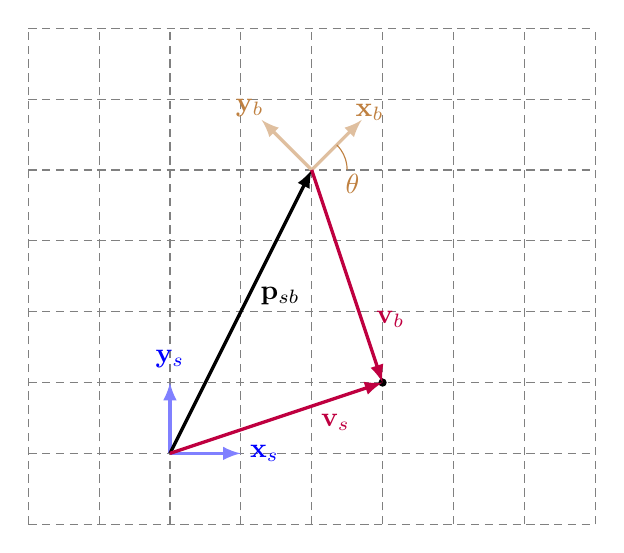
\begin{tikzpicture}[scale=4.5]
          \foreach \x in {-0.4, -0.2, 0, 0.2, 0.4, 0.6, 0.8, 1.0, 1.2}
            \draw[gray, thin, densely dashed] (\x,-0.2)--(\x,1.2);
          \foreach \x in {-0.2, 0, 0.2, 0.4, 0.6, 0.8, 1.0, 1.2}
            \draw[gray, thin, densely dashed] (-0.4,\x)--(1.2,\x);
          \draw[very thick, blue!50!, -latex] (0,0) -- (0.2,0) node[xshift=0.3cm, yshift=0cm, text=blue]{$\mf{x}_s$};
          \draw[very thick, blue!50!, -latex] (0,0) -- (0,0.2) node[xshift=0cm, yshift=0.3cm, text=blue]{$\mf{y}_s$};
          \draw[very thick, brown!50!, -latex] (0.4,0.8) -- (0.5414,0.9414) node[xshift=0.1cm, yshift=0.1cm, text=brown]{$\mf{x}_b$};
          \draw[very thick, brown!50!, -latex] (0.4,0.8) -- (0.2586, 0.9414) node[xshift=-0.15cm, yshift=0.15cm, text=brown]{$\mf{y}_b$};
          \draw[very thick, black, -latex] (0,0) -- (0.4,0.8) node[xshift=-0.4cm, yshift=-1.6cm]{$\mf{p}_{sb}$};
          \filldraw (0.6,0.2) circle (0.01cm);
          \draw[very thick, purple, -latex] (0,0) -- (0.6,0.2) node[xshift=-0.6cm, yshift=-0.5cm]{$\mf{v}_{s}$};
          \draw[very thick, purple, -latex] (0.4,0.8) -- (0.6,0.2) node[xshift=0.1cm, yshift=0.8cm]{$\mf{v}_{b}$};
          \draw[brown] (0,0) ++ (0.5,0.8) arc (0:45:0.1) node[xshift=0.2cm, yshift=-0.5cm]{$\theta$};
        \end{tikzpicture}
      \end{figure}
    \end{column}
  \end{columns}
\end{frame}


\begin{frame}{Rigid Body Motions in a Plane: Rotation and Translation}
  \begin{columns}[T]
    \begin{column}{0.475\textwidth}
      The pair $\lp \mf{R}_{sb}, \mf{p}_{sb}\rp$ allows:
      \begin{enumerate}
        \item Representation of a rotated and translated frame \rbframe{b} w.r.t \rbframe{s}.
        \item Transformation of vectors between \rbframe{s} and \rbframe{b}.
        \item Performs rotation and transalation of a give vector.
      \end{enumerate}
    \end{column}
    \begin{column}{0.5\textwidth}
      \begin{figure}
        \centering
        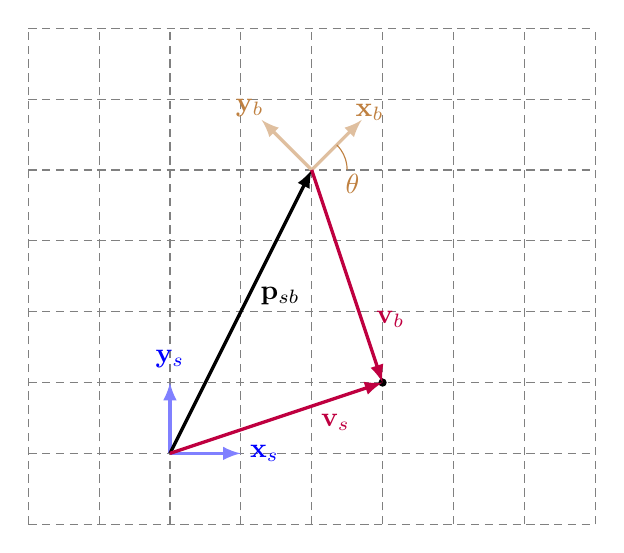
\begin{tikzpicture}[scale=4.5]
          \foreach \x in {-0.4, -0.2, 0, 0.2, 0.4, 0.6, 0.8, 1.0, 1.2}
            \draw[gray, thin, densely dashed] (\x,-0.2)--(\x,1.2);
          \foreach \x in {-0.2, 0, 0.2, 0.4, 0.6, 0.8, 1.0, 1.2}
            \draw[gray, thin, densely dashed] (-0.4,\x)--(1.2,\x);
          \draw[very thick, blue!50!, -latex] (0,0) -- (0.2,0) node[xshift=0.3cm, yshift=0cm, text=blue]{$\mf{x}_s$};
          \draw[very thick, blue!50!, -latex] (0,0) -- (0,0.2) node[xshift=0cm, yshift=0.3cm, text=blue]{$\mf{y}_s$};
          \draw[very thick, brown!50!, -latex] (0.4,0.8) -- (0.5414,0.9414) node[xshift=0.1cm, yshift=0.1cm, text=brown]{$\mf{x}_b$};
          \draw[very thick, brown!50!, -latex] (0.4,0.8) -- (0.2586, 0.9414) node[xshift=-0.15cm, yshift=0.15cm, text=brown]{$\mf{y}_b$};
          \draw[very thick, black, -latex] (0,0) -- (0.4,0.8) node[xshift=-0.4cm, yshift=-1.6cm]{$\mf{p}_{sb}$};
          \filldraw (0.6,0.2) circle (0.01cm);
          \draw[very thick, purple, -latex] (0,0) -- (0.6,0.2) node[xshift=-0.6cm, yshift=-0.5cm]{$\mf{v}_{s}$};
          \draw[very thick, purple, -latex] (0.4,0.8) -- (0.6,0.2) node[xshift=0.1cm, yshift=0.8cm]{$\mf{v}_{b}$};
          \draw[brown] (0,0) ++ (0.5,0.8) arc (0:45:0.1) node[xshift=0.2cm, yshift=-0.5cm]{$\theta$};
        \end{tikzpicture}
      \end{figure}
    \end{column}
  \end{columns}
\end{frame}


\begin{frame}{Rigid Body Motions in a Plane: Rotation and Translation}
  \begin{columns}[T]
    \begin{column}{0.475\textwidth}
      Find the pair $\lp \mf{R}_{sb_2}, \mf{p}_{sb_2}\rp$, given the pairs $\lp \mf{R}_{sb_1}, \mf{p}_{sb_1} \rp$ and $\lp \mf{R}_{b_1b_2}, \mf{p}_{b_1b_2} \rp$.
    \end{column}
    \begin{column}{0.5\textwidth}
      \begin{figure}
        \centering
        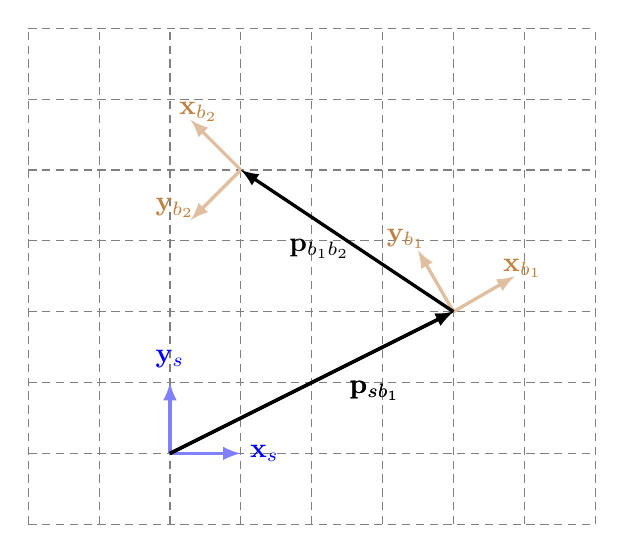
\begin{tikzpicture}[scale=4.5]
          \foreach \x in {-0.4, -0.2, 0, 0.2, 0.4, 0.6, 0.8, 1.0, 1.2}
            \draw[gray, thin, densely dashed] (\x,-0.2)--(\x,1.2);
          \foreach \x in {-0.2, 0, 0.2, 0.4, 0.6, 0.8, 1.0, 1.2}
            \draw[gray, thin, densely dashed] (-0.4,\x)--(1.2,\x);
          \draw[very thick, blue!50!, -latex] (0,0) -- (0.2,0) node[xshift=0.3cm, yshift=0cm, text=blue]{$\mf{x}_s$};
          \draw[very thick, blue!50!, -latex] (0,0) -- (0,0.2) node[xshift=0cm, yshift=0.3cm, text=blue]{$\mf{y}_s$};
          % Body frame 1
          \draw[very thick, brown!50!, -latex] (0.8,0.4) -- (0.973,0.5) node[xshift=0.1cm, yshift=0.1cm, text=brown]{$\mf{x}_{b_1}$};
          \draw[very thick, brown!50!, -latex] (0.8,0.4) -- (0.7, 0.5732) node[xshift=-0.15cm, yshift=0.15cm, text=brown]{$\mf{y}_{b_1}$};
          \draw[very thick, black, -latex] (0,0) -- (0.8,0.4) node[xshift=-1cm, yshift=-1cm]{$\mf{p}_{sb_1}$};
          % Body frame 2
          \draw[very thick, brown!50!, -latex] (0.2,0.8) -- (0.0586,0.9414) node[xshift=0.1cm, yshift=0.1cm, text=brown]{$\mf{x}_{b_2}$};
          \draw[very thick, brown!50!, -latex] (0.2,0.8) -- (0.0586, 0.6586) node[xshift=-0.2cm, yshift=0.15cm, text=brown]{$\mf{y}_{b_2}$};
          \draw[very thick, black, -latex] (0,0) -- (0.8,0.4) node[xshift=-1cm, yshift=-1cm]{$\mf{p}_{sb_1}$};
          \draw[very thick, black, -latex] (0.8,0.4) -- (0.2,0.8) node[xshift=1cm, yshift=-1cm]{$\mf{p}_{b_1b_2}$};
          
        \end{tikzpicture}
      \end{figure}
    \end{column}
  \end{columns}
\end{frame}


\begin{frame}{Rigid Body Motions in a Plane: Homogenous representation}
  \begin{itemize}
    \item The combined transformation of rotation and translation can be represented as a simple linear operation by using the homogenous representation for vectors and the transformations.
    \item For rotations and translations in $\mb{R}^2$, these rigid body transformations have a simple representation for the matrices and vectors in $\mb{R}^3$. The homogenous representation of a vector $\mf{r} \in \mb{R}^2$ is given by,
    \[ \overline{\mf{r}} = \bmx \mf{r} \\ 1\emx = \bmxc r_x \\ r_y \\ 1\emx \in \mb{R}^3\]
    \item The homogenous representation of rigid body transformation invovling a rotation $\mf{R} \in \mb{R}^{2 \times 2}$ and translation $\mf{p} \in \mb{R}^2$ is given by,
    \[ \overline{\mf{H}} = \bmx \mf{R} & \mf{p} \\ \mf{0} & 1 \emx \in \mb{R}^3 \]
  \end{itemize}
\end{frame}


\begin{frame}{Rigid Body Motions in a Plane: Homogenous representation}
  \begin{columns}[T]
    \begin{column}{0.5\textwidth}
      \[ \mf{p}_{sb} := \bmx p_{{sb}_x} \\ p_{{sb}_y} \emx \quad \quad \mf{R}_{sb} = \bmx \cos\theta  & \sin\theta \\ -
      \sin\theta & \cos\theta \emx \]

      The homogenous representation of the pair $\lp \mf{R}_{sb}, \mf{p}_{sb}\rp$ is given by, 
      \[ \overline{\mf{H}}_{sb} = \bmx \mf{R}_{sb} & \mf{p}_{sb} \\ \mf{0} & 1 \emx = \bmxc \cos\theta  & \sin\theta & p_{{sb}_x}\\ -
      \sin\theta & \cos\theta  & p_{{sb}_y} \\ 
      0 & 0 & 1\emx \]
      
    \end{column}
    \begin{column}{0.475\textwidth}
      \begin{figure}
        \centering
        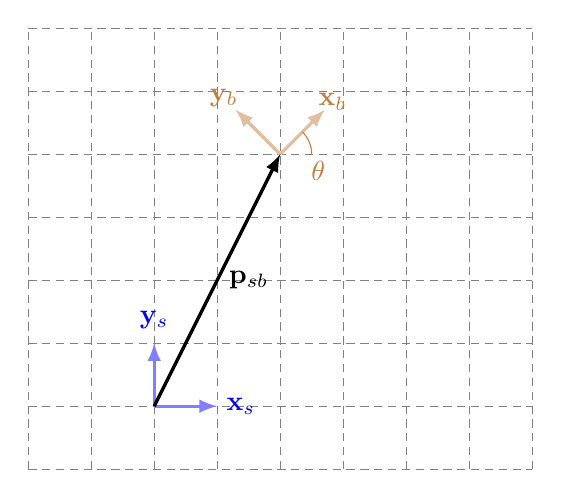
\begin{tikzpicture}[scale=4.0]
          \foreach \x in {-0.4, -0.2, 0, 0.2, 0.4, 0.6, 0.8, 1.0, 1.2}
            \draw[gray, thin, densely dashed] (\x,-0.2)--(\x,1.2);
          \foreach \x in {-0.2, 0, 0.2, 0.4, 0.6, 0.8, 1.0, 1.2}
            \draw[gray, thin, densely dashed] (-0.4,\x)--(1.2,\x);
          \draw[very thick, blue!50!, -latex] (0,0) -- (0.2,0) node[xshift=0.3cm, yshift=0cm, text=blue]{$\mf{x}_s$};
          \draw[very thick, blue!50!, -latex] (0,0) -- (0,0.2) node[xshift=0cm, yshift=0.3cm, text=blue]{$\mf{y}_s$};
          \draw[very thick, brown!50!, -latex] (0.4,0.8) -- (0.5414,0.9414) node[xshift=0.1cm, yshift=0.1cm, text=brown]{$\mf{x}_b$};
          \draw[very thick, brown!50!, -latex] (0.4,0.8) -- (0.2586, 0.9414) node[xshift=-0.15cm, yshift=0.15cm, text=brown]{$\mf{y}_b$};
          \draw[very thick, black, -latex] (0,0) -- (0.4,0.8) node[xshift=-0.4cm, yshift=-1.6cm]{$\mf{p}_{sb}$};
          \draw[brown] (0,0) ++ (0.5,0.8) arc (0:45:0.1) node[xshift=0.2cm, yshift=-0.5cm]{$\theta$};
        \end{tikzpicture}
      \end{figure}
    \end{column}
  \end{columns}
\end{frame}


\begin{frame}{Rigid Body Motions in a Plane: Rotation and Translation}
  \begin{itemize}
    \item The inverse of the rigid body transformation $\homo{H}{sb}$ is given by,
    \[ \homo{H}{bs} = \homo{H}{sb}^{-1} = \bmxc \mf{R}_{sb}^\top & -\mf{R}_{sb}^\top\mf{p}_{sb} \\ \mf{0} & 1 \emx \]

    \item Verify that $\homo{H}{sb}\homo{H}{bs} = \homo{H}{bs}\homo{H}{sb} = \mf{I}_3$.

    \item What is the interpretation of $-\mf{R}_{sb}^\top\mf{p}_{sb}$?
    
    \item What are the homogenous representations of a pure rotation and a pure translation?
  \end{itemize}
\end{frame}


\begin{frame}{Rigid Body Motions in 3D: Rotation}
  \begin{columns}[T]
    \begin{column}{0.475\textwidth}
      The representation of \rbframe{b} in \rbframe{s} is given the following,
      \[ \mf{R}_{sb} = \bmxc 
      \mf{x}_{s}^\top \mf{x}_{b} & \mf{x}_{s}^\top \mf{y}_{b} & \mf{x}_{s}^\top \mf{z}_{b}\\
      \mf{y}_{s}^\top \mf{x}_{b} & \mf{y}_{s}^\top \mf{y}_{b} & \mf{y}_{s}^\top \mf{z}_{b}\\
      \mf{z}_{s}^\top \mf{x}_{b} & \mf{z}_{s}^\top \mf{y}_{b} & \mf{z}_{s}^\top \mf{z}_{b}
      \emx \in \mb{R}^{3 \times 3} \]
    \end{column}
    \begin{column}{0.5\textwidth}
      \begin{figure}
        \centering
        \tdplotsetmaincoords{45}{135} % Set the viewpoint angle
        \begin{tikzpicture}[scale=3, tdplot_main_coords]
            % Draw the first reference frame
            \draw[thick,-latex] (0,0,0) -- (1,0,0) node[anchor=north east]{$\mf{x}_{s}$};
            \draw[thick,-latex] (0,0,0) -- (0,1,0) node[anchor=north west]{$\mf{y}_{s}$};
            \draw[thick,-latex] (0,0,0) -- (0,0,1) node[anchor=south]{$\mf{z}_{s}$};
            
            % Rotate the viewpoint for the second reference frame
            \tdplotsetrotatedcoords{10}{20}{10}
            
            % Draw the second reference frame
            \begin{scope}[tdplot_rotated_coords]
                \draw[thick, red,-latex] (0,0,0) -- (1,0,0) node[anchor=north east]{$\mf{x}_{b}$};
                \draw[thick, red,-latex] (0,0,0) -- (0,1,0) node[anchor=north west]{$\mf{y}_{b}$};
                \draw[thick, red,-latex] (0,0,0) -- (0,0,1) node[anchor=south]{$\mf{z}_{b}$};
            \end{scope}
        \end{tikzpicture}
      \end{figure}
    \end{column}
  \end{columns}
\end{frame}


\begin{frame}{Rigid Body Motions in 3D: Rotation}
  \textbf{Properties of rotation matrices:}
  \begin{itemize}
    \item Inverse of a rotation matrix $\mf{R}$ is its transpose. $\mf{R}^\top = \mf{R}^{-1}$. This means that the columns of a rotation matrix are orthonormal.
    \item The determinant of a rotation matrix is always 1. $\det\lp \mf{R} \rp = 1$.
    \item The set of all 3D rotation matrices form a \textit{group} called the \textbf{\textit{Special Orthogonal}} group called the $SO\lp 3\rp$ group.
    \[ SO\lp 3 \rp := \lc \mf{R} \in \mb{R}^{3 \times 3} \, : \, \mf{R}^\top\mf{R} = \mf{I}, \, \det \mf{R} = +1 \rc  \]

    $SO\lp 3 \rp$ group is also referred to as the \textit{rotation group} of $\mb{R}^3$.
  \end{itemize}
\end{frame}



\end{document}